(i) The bar graph representing the above data is shown in figure \ref{fig:bar37_py}\\
\begin{figure}[!ht]
\centering
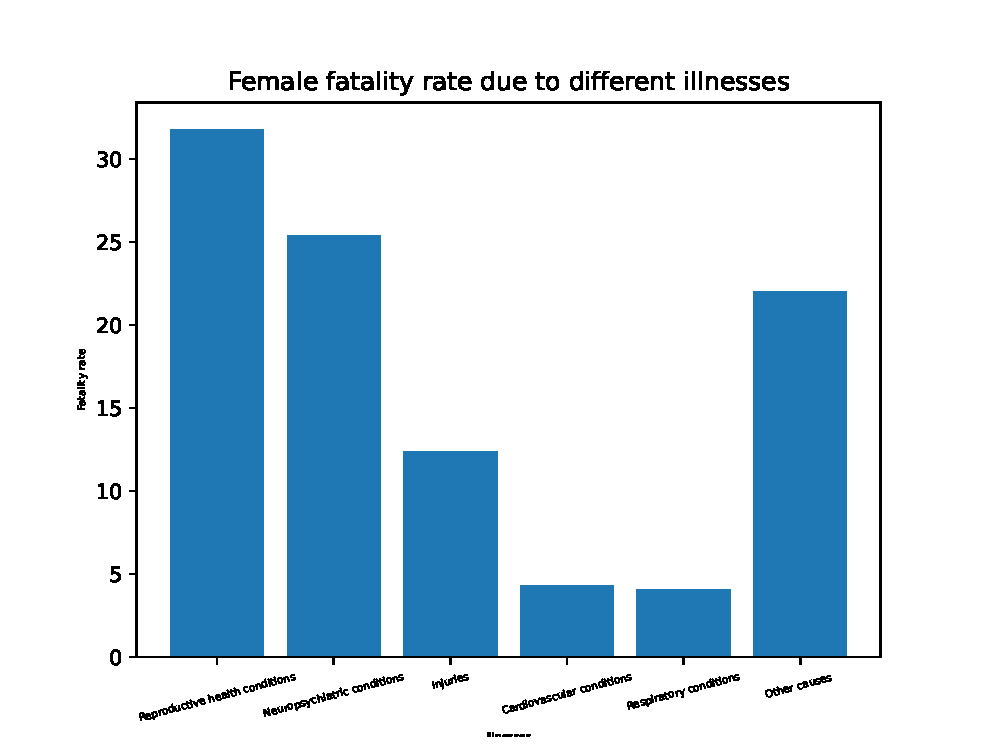
\includegraphics[width=\columnwidth]{./solutions/20-10/stat/codes/pyfigs/exer37.eps}
\caption{Illnesses and respective fatality rates amongst women}
\label{fig:bar37_py}
\end{figure}
(ii)Reproductive health conditions is the major cause of women's illness and death.\\
(iii)Lack of awareness and understanding about reproductive health results in high female fatality rate due to reproductive health conditions.\\
The python code used to generate the bar graph \ref{fig:bar37_py} is
\begin{lstlisting}
./solutions/20-10/stat/codes/exer37.py
\end{lstlisting}
